\documentclass[12pt,a4paper,oneside]{report}
\usepackage{indentfirst}
\usepackage{times}
\setlength\parindent{1cm}
\renewcommand{\baselinestretch}{1.50}\normalsize
\usepackage{anysize}
\marginsize{1.25in}{.75in}{1in}{1in}
\usepackage{graphics}
\usepackage{graphicx}
\usepackage{epsfig}
\usepackage[fleqn]{amsmath}
\usepackage{amsfonts}
\usepackage{textcomp}
\usepackage{graphicx}
\usepackage{setspace}
\usepackage{fancyhdr}
\usepackage{truncate}
\usepackage{nomencl} 
\usepackage{acronym}
\usepackage{array}
\usepackage{caption}
\usepackage{subfig}
\usepackage[overload]{textcase}
\usepackage{listings}
\renewcommand{\nomname}{List of Abbreviations}
\usepackage{makeidx}
\makeindex
\makenomenclature
\newcommand{\quotes}[1]{``#1''}
\usepackage{titlesec}
\titleformat{\chapter}[display]
{\normalfont\Large\bfseries\centering}
{\chaptertitlename\ \thechapter}{15pt}{\LARGE}
\titleformat{\section}{\large\bfseries}{\thesection}{1em}{}
\titleformat{\subsection}{\normalsize\bfseries}{\thesubsection}{1em}{}
\renewcommand{\chaptermark}[1]{\markboth{ \emph{#1}}{}}

\printnomenclature[5em]
\pagestyle{fancy}
%\headheight 1pt
	\renewcommand{\footrulewidth}{1.2pt}
\renewcommand{\headrulewidth}{1.2pt}
\rhead{\scriptsize {\leftmark}}

\lhead{\small{College of Engineering, Cherthala \;\;\;\;\;\;\;\;\;\;\;\;\;\;\;\;\;\;}}
\rfoot{\thepage}
\cfoot{\empty}
\lfoot{\small{Department of Computer Science \& Engineering}}
\renewcommand{\figurename}{Fig.}
\begin{document}
\renewcommand\bibname{References}
\begin{titlepage}
\begin{center}
\Large{\textbf{MAJOR PROJECT REPORT}}\\
\vspace{.2 in}
\begin{singlespace}
\LARGE{\textbf{EBA - Electricity Board Application }}\\
\end{singlespace}
\vspace{.1 in}
\Large{\textit{Submitted By }}\\
\Large{\textit{\textbf{AJESH M (Reg. No. 12141201)}}} \\
\Large{\textit{\textbf{MUHAMMED NADIRSHA (Reg. No. 12143615)}}} \\
\Large{\textit{\textbf{RIBIN ROY (Reg. No. 12143620)}}} \\
\Large{\textit{\textbf{SREENIVAS S NAIK (Reg. No. 121436)}}} \\
\Large{\textit{\textit{under the guidance of}}}\\
\Large{\textit{Mrs. Anitha M. A.}}\\
\Large{\textit{(Assistant Professor)}}\\
\Large{\textit{Computer Science \& Engineering}}
\vspace{.05in}
\begin{figure}[h]
\begin{center}

\epsfig{width=1.5 in, file=logo.jpg}
\end{center}
\end{figure}
\begin{singlespace}
\large{\textbf{MARCH 2017}}\\
\vspace{.1in}
\large{\textbf{DEPARTMENT OF COMPUTER SCIENCE AND ENGINEERING\\COLLEGE OF ENGINEERING,CHERTHALA\\ PALLIPPURAM P O, ALAPPUZHA-688541, \\PHONE: 0478 2553416, FAX: 0478 2552714\\http://www.cectl.ac.in}}
\end{singlespace}
\end{center}
\end{titlepage}

\begin{titlepage}
\begin{center}

\large{\textbf{MAJOR PROJECT REPORT}}\\
\begin{singlespace}
\LARGE{\textbf{EBA - Electricity Board Application }}\\
\end{singlespace}


\Large{\textit{Submitted By }}\\
\Large{\textit{\textbf{AJESH M (Reg. No. 12141201)}}} \\
\Large{\textit{\textbf{MUHAMMED NADIRSHA (Reg. No. 12143615)}}} \\
\Large{\textit{\textbf{RIBIN ROY (Reg. No. 12143620)}}} \\
\Large{\textit{\textbf{SREENIVAS S NAIK (Reg. No. 121436)}}} \\
\Large{\textit{\textit{under the guidance of}}}\\
\Large{\textit{Mrs. Anitha M. A.}}\\
\begin{singlespace}
\large{\textit{In partial fulfillment of the requirements for the award of the degree}\\
\large{ \textit{of}}\\
\large{\textit{Bachelor of Technology} }\\
\large{\textit{in}}\\
\large{\textit{Computer Science and Engineering}}\\
\large{\textit{of}}\\
\large{\textit{Cochin University Of Science And Technology }}}\\
\end{singlespace}
\begin{figure}[h]
\begin{center}

\epsfig{width=0.6in, file=logo.jpg}
\end{center}
\end{figure}
\begin{singlespace}

\Large{\textbf{MARCH 2017\\Department of Computer Science and Engineering\\College of Engineering, Pallippuram P O, Cherthala, Alappuzha Pin: 688541, \\Phone: 0478 2553416, Fax: 0478 2552714\\http://www.cectl.ac.in}}
\end{singlespace}
\end{center}
\end{titlepage}


\begin{titlepage}
\begin{center}

\large{\textbf{DEPARTMENT OF COMPUTER SCIENCE \& ENGINEERING}}\\
\large{\textbf{COLLEGE OF ENGINEERING CHERTHALA\\ALAPPUZHA-688541}}\\
\end{center}
\begin{figure}[h]
\begin{center}

\epsfig{width=1.5in, file=logo.jpg}
\end{center}
\end{figure}
\begin{center}
\large{\textbf{C E R T I F I C A T E}}\\
\end{center}
\begin{spacing}{1.5}
\par This is to certify that, the Major Project Report submitted by \\

\par In partial fulfilment of the requirement of course of the Bachelor of Technology, (B. Tech)in Computer Science \& Engineering prescribed by Cochin University of Science \& Technology during the academic year 2016-2017\\ 
\end{spacing}
\begin{tabbing}
xxxxxxxxxxxxxxxxxxxxxxxxxxxxxxxxxxxxxx\= xxxxxxxxxxxxxxxxxxxx\= \kill
\hspace{.4in}{\bf Guide} \>\hspace{-.5in}{\bf Co-ordinator}\hspace{1.7in}{\bf  HoD  } \\
\end{tabbing}
\begin{tabbing}
xxxxxxxxxxxxxxxxxxxxxxxxxxxxxxxxxxxxxx\= xxxxxxxxxxxxxxxxxx\= \kill
%\vspace{0.3in}\\
\hspace{.15in}{\bf{Mrs. Anitha M. A.}}   \>\hspace{-.7in}{\bf Mr. Muhammed Ilyas H} \hspace{.65 in}{\bf Dr. Preetha Theresa Joy }\\
\hspace{.15in}Assistant Professor    \>\hspace{-.7in}Assistant Professor\>\hspace{.23in}Professor\\
\hspace{.1in} Computer Science\&Engg    \>\hspace{-.75in}    Computer Science\&Engg \>\hspace{.18in}    Computer Science\&Engg\\

\end{tabbing}
\end{titlepage}

  \newpage
  \section*{\begin{center}\Large ACKNOWLEDGEMENT\end{center}}
  \thispagestyle{empty}
  \par
  \hspace{0.1in}
 \par  We take this opportunity to express our sincere gratitude to the people who have been instrumental in the successful completion of our major project.\\
 \par  For every endeavour in our life, the help of the Lord has always followed. We have yet again experienced his loving kindness while preparing for this project. We would like to express our sincere thanks to the Principal, \textbf{Dr. Mini M. G} , for her valuable support and advice. We would also like to thank our Head Of Computer Science Department, \textbf{Dr. Preetha Theresa Joy} for her support. We express our heartfelt gratitude to our project coordinator, \textbf{Mr. Muhammed Ilyas H} (Assistant Professor, Department of Computer Science) for his valuable help and support. We would also like to thank our project Guide, Mrs. Fathima N (Assistant Professor, Department of Computer Science) for her support and guidance.\\
 \par We are indebted to all teaching and non-teaching staff of the Department of Computer Science \& Engineering, friends and family for their co-operation and support, with out which we could never have completed the project this well.\\
 
 \newpage
 \section*{\begin{center}\Large ABSTRACT\end{center}}
 \thispagestyle{empty}
 \par
 \hspace{0.1in}
 \par The User Assistance Chatbot project is built using artificial algorithms that analyses users queries and understand users message. This System is a web application which provides answer to the query of the user. Users just have to query through the bot which is used for chating. Users can chat using any format there is no specific format the user has to follow. The System uses built in artificial intelligence to answer the query. The answers are appropriate to what the user queries. The System analyses the question and then answers to the user. The system answers to the query as if it is answered by the person. With the help of artificial intelligence, the system answers the query asked by the students. The system replies using an effective graphical user interface which implies that as if a real person is talking to the user. The user just has to register himself to the system and has to login to the system. After login user can access to the various helping pages. Various helping pages has the bot through which the user can chat by asking queries . The system replies to the user with the help of effective graphical user interface.
 
\tableofcontents
\pagenumbering{roman}
\listoffigures


\def\addsymbol #1: #2#3{\;\;\;\;\;\;\;\;\;\;\;\;\;\;\;\;\;\;\;\;\;\;\;$#1$ \> \;\;\;\;\;\;\;\;\;\;\;\;\;\;\;\;\;\;\;\;\;\;\;\;\;\; \parbox{5in}{#2}\\}



\renewcommand*\thesection{\thechapter.\arabic{section}}
\newpage
\pagestyle{fancy}
%\headheight 2pt
\renewcommand{\footrulewidth}{1.2pt}
\renewcommand{\headrulewidth}{1.2pt}
\rhead{\scriptsize {\leftmark}}
%\chead{Middle top}
\lhead{\small{College of Engineering, Cherthala \;\;\;\;\;\;\;\;\;\;\;\;\;\;\;\;\;\;}}
\rfoot{\thepage}
\cfoot{\empty}
\lfoot{\small{Department of Computer Science \& Engineering}}


\chapter{INTRODUCTION}
\label{intro}
\pagenumbering{arabic}
\setcounter{page}{1}
%\hspace{0.1in}
\section{PURPOSE}
\par 
A chatbot is a type of conversational agent designed to simulate an intelligent conversation with one or more humans by an auditory or textual methods. The User Assistance Chatbot is built using artificial algorithms that analyses users queries and understand users message. This system is a web application which provides answer to the query of the user. Users can input documents like pdf, ebook, etc and then to retrive any information, the user just have to query through the bot which is used for chating. The system uses built in artificial intelligence to answer the query. The answers are appropriate to what the user queries. The system replies using an effective graphical user interface which implies that as if a real person is talking to the user. The user just has to register himself to the system and has to login to the system. After login user can access to the various helping pages. Various helping pages has the bot through which the user can input the document and chat by asking queries. The system replies to the user with the help of effective graphical user interface.


\section{SCOPE}
\par Searching for an information in a large document is time consuming and is a difficult process. It needs lot of effort from the user. This application makes the search process more easier. Users can easily login to the page. Documents like pdf file or ebook can be given as the input. User can ask any queries related to the document given as input. The bot replies precisely as if a real person is answering. Bots are going to explore and the phenomenon is sure to run through into the foreseeable future- and there is no question thet they are already dominating the news right now. A chatbot is eseentially a computer program that simulates human conversation or chat through artificial intelligence(AI). It is extensively used in applications such as e-commerce, call centre and internet gaming.\\
\par The first and foremost emphasis in regard to the messenger bot should be the fact that it should connect people and bridge the contrasts of the society, effectively and essentially. One of the trending example for the same is messenger processing is around 60 billion messages per day while global SMS volume was around 20 billion messages per day.\\ 
\par Chatbots conducts a conversation via auditory or textual methods. Such programs are often designed to convincingly simulate how a human would behave as a conversational partner, thereby passing the turing test. Chatbots are typically used in dialogue systems for various practical purposes including customer service or information acquisition. Some chatbots use sophisiticated natural language processing systems, but many simpler systems scans for keywords within the input, then pull a reply with the most matching keywords, or the most similar word in pattern from a dtabase. THere are two main types of chatbots, One functions baesd on a set of rule, and the other more advanced version uses artificial intelligence. The chatbots based on rules, tend to be limited in functionality, and are as smart as they are programmed to be. On the other end, a chatbot that uses AI understands language, not just commands, and continuously gets smarter as it learns from conversations it has with people.\\
\chapter{SYSTEM ANALYSIS}

%\hspace{0.1in}

\section {EXISTING SYSTEM}
The existing systems are:
\begin{itemize}
\item ELIZA- It is a web robot and can conduct dialogs with humans through a web interface. It is based on very simple pattern recognition and on a stimulus response model.
\item ALICE- It is a natural language processing chatbot. It applys some pattern matching rules to the users query and then generate an appropriate response.
\end{itemize}
\par  The existing chatbot systems are used mainly for the purpose of chatting with the user. They are mainly used for casual communication with user. 

\subsection {PROPOSED SYSTEM}
The chatbot is trained in such a way that it answers to the queries of user, related to the document given as input to the system. The user don't have to waste the time by reading whole document instead the bot will answer the queries. The output will be available in the form of both text and speech. The system provides precise output to its user.
%\newpage
\subsection {PRODUCT FUNCTIONS}
\begin{itemize}
 \item It helps to reduce the burden of user, who has to read a large document inorder to retrive any information from it.
 
\item The output will be available in the form of both text and speech.
\end{itemize}

\section{LIFE CYCLE MODEL}
\par The paradigm chosen for this project is prototype life cycle model. Prototype model should be used when the desired system needs to have a lot of interaction with the end users. Prototype ensures that the end users constantly works with the system and provide a feedback which is incorporated in the prototype to result in a usable system. They are excellent for designing good human computer interface systems. For the entire graphical user interfacing prototype life cycle model is used. The basic idea here is that instead of freezing the requirements before a design or coding can proceed, a through way prototype is built to understand the requirements. By using this prototype, the client can get an “actual feel” of the system, since the interactions with the prototype can enable the client to better understand the requirements of the desired system. Prototyping is an attractive idea for complicated and large systems for which there is no manual processor existing system to help determining the requirements. The prototype is usually not complete systems and many of the details are not built in the prototype. The goal is to provide a system with overall functionalities.\\
\par Users are actively involved in the development. Since in this methodology a working model of the system is provided, the users get a better understanding of the system being developed. Errors can be detected much earlier. Quicker user feedback is available leading to better solutions. Missing functionality can be identified easily. Confusing or difficult functions can be identified. Required validation, quick implementation of, incomplete, but functional, application.\\
\par  As a part of applying prototyping in our project, first we generated a rough interface of our UBO. Later on, based on the requirements alterations were made. After the customer accepts rest comes the design phase, coding, testing and then maintenance. The disadvantages of the prototype life cycle model is developing time is high and compromising in the quality and performance of the product for the sake of the customer’s satisfactions. Since the developing time is high in this type of life cycle, the developing cost is will also be high.
\section{FEASIBILITY STUDY}
\par The main objective of this study is to determine whether the proposed system is feasible or not. Mainly there are three types of feasibility study to which the proposed system is subjected as described below: Four key considerations are involved in this feasibility.\\
\begin{itemize}
\item Economic Feasibility
\item Technical Feasibility
\item Operational Feasibility
\item Social Feasibility
\end{itemize}
The proposed system must be evaluated from a technical viewpoint first, and if technically feasible, their impact on the organization must be assessed. If compatible, the operational system can be devised. Then those must be tested for economic feasibility.
\subsection{Technical Feasibility}
The technology required for developing the driver is identified. It has technical capability to initialize the system and perform data transfer. It also provides technical guarantee of assurance,reliability,easy access and security. Thus,since both hardware and software requirements are satisfied it is technically feasible.
\subsection{Economical Feasibility}
The system is developed at reasonable cost with the available hardware, software and manpower. So its benefits overweigh the cost. So it is economically feasible.
\subsection{Operational Feasibility}
The proposed project is beneficial because this driver software is the first of its class, so the users are encouraged to use it, and is expected to serve the user’s needs on request. The user interface is designed in such a way that the users are not bound to have any doubts to use the interface.
\subsection{Social feasibility}
The proposed project will be socially feasible as the contents being shared is only inside a friend’s circle. Such that it would not be used for any offensive purposes. The social feasibility determines whether the project would be accepted by the people. This assumption would in general examine the probability that the project would have to be accepted by the group of people that are directly affected by the proposed system.

\section{GANTT CHART}
\par Gantt chart is a graphical representation of allocation of resources to the activities. Here our resource is time. A Gantt chart is a type of bar chart that illustrates a project schedule. Gantt charts illustrate the start and finish dates of the terminal elements and summary elements of a project. Terminal elements and summary elements comprise the work breakdown structure of the project. Some Gantt charts also show the dependency (i.e., precedence network) relationships between activities. 
\par Gantt charts have become a common technique for representing the phases and activities of a project work breakdown structure (WBS), so they can be understood by a wide audience. Although a Gantt chart is useful and valuable for small projects that fit on a single sheet or screen, they can become quite unwieldy for projects with more than about 30a ctivities. Larger Gantt charts may not be suitable for most computer displays. A related criticism is that Gantt charts communicate relatively little information per unit area of display. That is, projects are often considerably more complex than can be communicated effectively with a Gantt chart. Although project management software can show schedule dependencies as lines between activities, displaying a large number of dependencies may result in a cluttered or unreadable chart. \\
\par Because the horizontal bars of a Gantt chart have a fixed height, they can misrepresent the time- phased work load (resource requirements) of a project, which may cause confusion especially in large projects. A related criticism is that all activities of a Gantt chart show planned workload as constant. In practice, many activities (especially summary elements) have front loaded or back-loaded work plans,so a Gantt chart with percent-complete shading actually may lead to miscommunications on the true schedule performance status.
\begin{figure}[h]
	\begin{center}
		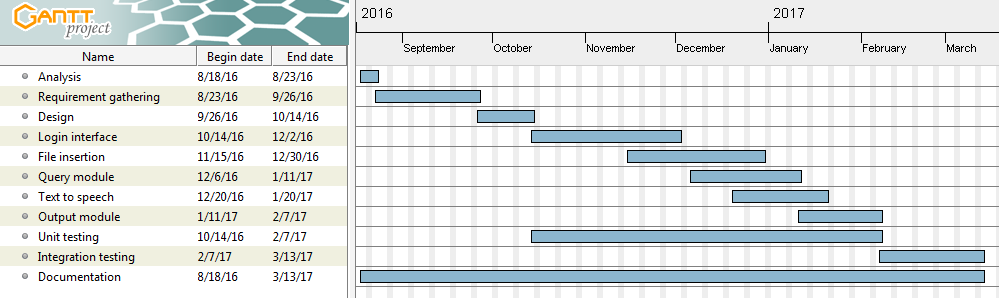
\includegraphics[width=16cm,height=7cm]{abcdgantt.png}
			\caption{Gantt Chart}
			\label{Gantt Chart}
	\end{center}
\end{figure}
In the Gantt Chart, as per the module name each dates are given. For the feasibility study five days are given and parallel to that the requirement analysis has been started. After this comes the design phase, during this phase it took for over eighteen days for coming up with the suitable design interface according to our project. Next as a part of the implementation stage it took fourty eight days for GUI development. Then comes the implementation of each modules according to our project. First in the File Insertion Module it took fourty five days for its completion and for Query module it took twenty eight days and our last module that is the Text to Speech module it took twelve days for its completion. Rest comes the testing phase for double checking the performance analysis of our project by underlying them over various perspective by Unit testing, Integration testing, Final testing. At last comes the thorough documentation of each and every nook and corner of the project done, evaluated and analysed.

\section{COSTESTIMATION}
\par Basic COCOMO computes software development effort (and cost) as a function of program size. Program size is expressed in estimated thousands of lines of code (KLOC).\\
\par COCOMO applies to three classes of software projects:\\

\begin{itemize}
\item Organic projects - \quotes{small} teams with \quotes{good} experience working with \quotes{less than rigid} requirements
\item Semi-detached - \quotes{medium} teams with mixed experience working with a mix of rigid and less than rigid requirements
\item Embedded projects - developed within a set of \quotes{tight} constraints (hardware, software, operational ...)
\end{itemize}
\par The basic COCOMO equations take the form:\\ 
\par Effort Applied = $a(KLOC)^b$[ person-months ]\\
\par Development Time = $c(EffortApplied)^d$[months]\\
\par People required = $Effort Applied / Developmen Time$ [count]\\
\par The coefficients a, b, c and d are given in the following table.\\
\begin{figure}[h]
	\begin{center}
		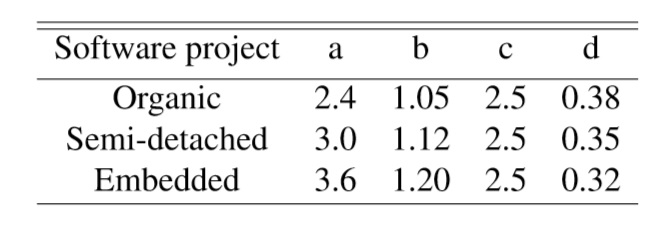
\includegraphics[width=13cm,height=5cm]{cocomotable.jpg}
			\caption{ COCOMO Model Coefficients}
			\label{ COCOMO Model Coefficients}
	\end{center}
\end{figure}
\textit{Cost Estimation of Our Project:}\\
Effort for Development: 6PM \\
Time for development is expected to be 3 months\\
\section{SYSTEM REQUIREMENT STUDY}
\subsection{ Hardware Requirements}
\par The recommended minimum system should have 2 GHz processor,500 MB RAM,and disk space as required.\\
\subsection{ Software Requirements}
\begin{itemize}
\item Tools : PyCharm IDE
\item Front End : HTML, Python
\item Back End : MySQL, AIML
\item Database : MySQL
\item Platform : Windows, Linux
\item Web browser : Internet Explorer 6.0 or above

\end{itemize}
\subsection{Safety Requirements}
\par Complete access to the system is allowed only to the administrator of this system. Clients can do nothing other than using the applications provided.\\
 
 
\chapter{SYSTEM DESIGN}
\section{DESIGN}
Design of the system includes mainly two steps:
\begin{itemize}
\item{System design}
\item{Detailed design}
\end{itemize}

 In System design a structural framework for the entire system is created. It is done in
such a way that related part come under particular groups. Thus after the system design, a
network of different groups is obtained. It is the high-level strategy for solving the problem
and building a solution. It includes the decision about the organization of the system into
subsystems, the allocation of subsystems to hardware and software components, and major
conceptual and policy decisions that form the framework for the detailed design.
\par In detailed design, each group is studied in detail and the internal operations are decided.
Based on this, the data structures and the programming language to be used are decided. Apart
from detailed design, the system design can be grouped into physical design and structural
design. The physical design maps out the details of the physical system and plans the system
implementation and specifies the hardware and software requirements.
\par Structured design is an attempt to minimize the complexity and make a problem manageable
by subdividing into smaller segments, which is called modularization or decomposition.
In this way structuring minimizes intuitive reasoning and promotes maintainable provable of systems. The structured design partitions a program into small, independent modules. They
are arranged in a hierarchy that approximates a model of the business are and is organized in a
top-down manner.
\par Logical design proceeds in a top-down manner. General features, such as reports and
inputs are identified first. Then each is studied individually and in more detail. Hence the
structured design is an attempt to minimize the complexity and make a problem.

\section{MODULES}
UBO can be divided  into the following modules.
\begin{itemize}
\item{Secure login interface.}
\item{Source file insertion module. }
\item{Query module.}
\item{Text to speech conversion.}
\item{Output module.}
\subsection{SECURE LOGIN INTERFACE}
\par This is the first module of the UBO. This feature will give the user a secure and simple login screen. The user will be provided
with a username and password by the administrator after verifying the credentials, which should
be used here.
\subsection{SOURCE FILE INSERTION MODULE}
This feature will allow the user to input the documents like pdf, ebook etc.
\subsection{QUERY MODULE}
This feature will allow the user to ask questions related to the inputted document. The
query is analysed by the chatbot and the answer is extracted from the database, where the input
is stored.
\subsection{TEXT TO SPEECH CONVERSION}
This feature converts the answer obtained in text form to voice output.
\subsection{OUTPUT MODULE}
The output is obtained in both text and voice format. Voice control mechanisms help in
varying the speed, pitch, loudness etc. of the output.
\end{itemize}
\section{USE CASE DIAGRAM}
\subsection{Purpose}
Use case diagram in the Unified Modelling language (UML) is a type of behavioural
diagram. Its purpose is to represent the graphical overview of the functionality provided by a
system in terms of actors, their goals (represented use cases), and any dependencies between
those use cases. The main purpose of a use case diagram is to show what system functions are
performed for which actor.\\
\newpage
\subsection{Diagram}
\begin{figure}[h]
  	\begin{center}
  		\includegraphics[width=5 in,height=4 in]{Usecase.png}
  			\caption{USE CASE Diagram}
  			\label{USE CASE Diagram}
  	\end{center}
  \end{figure}
\subsection{Description}
USER:
\begin{itemize}

\item{Login to the system through the first page of the application with his/ her unique username
and password.}
\item{Input a doccument}
\item{Ask queries about the document.}
\item{logout when the action is completed.}
\end{itemize}
\newpage
SERVER:
\begin{itemize}
\item{Search the database for the answers.}
\item{Bot gives answer to the queries in textual and speech form.}
\end{itemize}
\section{SEQUENCE DIAGRAM}
\subsection{Purpose}
A Sequence diagram depicts the sequence of actions that occur in a system. It portrays the
different perspectives of behaviour of the system and different types of inferences can be drawn
from them. The invocation of methods in each object, and the order in which the invocation
occurs is captured in a Sequence diagram. This makes the Sequence diagram a very useful tool
to easily represent the dynamic behaviour of a system.\\
\subsection{Diagram}
\begin{figure}[h]
  	\begin{center}
  		\includegraphics[width=4 in,height=3 in]{sequence.png}
  			\caption{SEQUENCE Diagram}
  			\label{SEQUENCE Diagram}
  	\end{center}
  \end{figure}
 \newpage
\subsection{Description}
After successful authentication with his/ her unique username and password, the user will
be able to upload the pdf . After uploading pdf user can ask queries about the contend of the pdf. The server stores the file in the data base at the same time. While user ask queries about the pdf server search for the answers from the database.And the appropriate answer is given to the user in both textual and speech form. The action is completed when
user logout from the system.

\section{ACTIVITY DIAGRAM}
\subsection{Purpose}
The basic purpose of activity diagrams are similar to other four diagrams. It captures the dynamic behaviour of the system. Other four diagrams are used to show the message flow from one object to another. But activity diagram is used to show message flow from one activity to another. Activity diagram is an important diagram in UML to describe dynamic aspects of the
system. Activity diagram is basically a flow chart to represent the flow form one activity to
another activity. The activity can be described as an operation of the system. So the control flow
is drawn from one operation to another. This flow can be sequential, branched or concurrent.
Activity diagrams deals with all type of flow control by using different elements like fork, join
etc. Activity is a particular operation of the system. Activity diagrams are not only used for visualizing dynamic nature of a system but they are also used to construct the executable system by using forward and reverse engineerig technique. The only missing thing in the avtivity diagram is the message part,. It doesnot show any flow from one activity to another. Activity diagram is sometimes considered as the flow chart. Although diagram looks like the flow chart but it is not. It shows different flow like parallel, branched, concurrent and single.\\
\newpage
\subsection{Diagram}
\begin{figure}[h]
  	\begin{center}
  		\includegraphics[width=4 in,height=5 in]{activity.png}
  			\caption{ACTIVITY Diagram}
  			\label{ACTIVITY Diagram}
  	\end{center}
  \end{figure}
 \newpage
\subsection{Description}
\par User login to the web page by using his/her user name and password. After successful login user can input the document and ask queries related to the inputted document. If the user is a new member he has to sign up using necessary informations. If the query is valid the bot will give answers by searching the database. User can  logout when the actions are completed.\\ 
\section{ER DIAGRAM}
\subsection{Purpose}
Database is recognized as a standard and is available virtually for every computer system.
The general theme behind every database is to integrate all the information. The database is an
integrated collection of data and provides centralized access to the data. The user authentication
in the project and share details is implemented using the database.
\subsection{Diagram}
\begin{figure}[h]
  	\begin{center}
  		\includegraphics[width=3 in,height=2 in]{Erdiagram.png}
  			\caption{ER Diagram}
  			\label{ER Diagram}
  	\end{center}
  \end{figure}
  \newpage
\subsection{Description}
The entity document has two attributes doc\_no and doc\_files, where doc\_no is the primary key. T
he entity user has two attributes user\_id and password, where user\_id is the primary key. User inputs document and chat bot give answers to the queries asked by user.
\section{DATA FLOW DIAGRAM}
\subsection{Purpose}
A data flow diagram is a simple graphical formalism that represents a system in terms
of the input data to the system, various processing carried on these data, and the output data
generated by the system. A DFD model represents the data flow aspects and does not show
the sequence of execution of the different functions and conditions based on which a function
may or not be executed .In fact it completely ignores aspects such as control flow, the specific
algorithms used by the functions etc.
A DFD model uses a very limited number of primitive symbols to represent the functions
performed by the system and data flow among these functions. This network is constructed
by using a set of symbols that do not imply a physical implementation. It is a graphical tool
for structured analysis of the system requirements. DFD models a system by using external
entities, from which data flows to a process, which transforms the data and creates, outputdata-
flows which go to other processor or external entities or files. Data in files may also flow
to processes as inputs.\\
\\
\textbf {Notation used in data flow}
\begin{itemize}
\item\textbf{Process}
\end{itemize}
\par Process shows the work of the system. Each process has one or more data inputs and produce one or more data outputs. Processes are represented by rounded rectangles in
Data Flow Diagram. Each process has a unique name and number. This name and
number appears inside the rectangle that represents the process in a Data Flow Diagram.\\
\begin{figure}[h]
  	\begin{center}
  	
  	
  		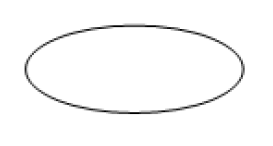
\includegraphics[width=3 in,height=1 in]{ellipse.png}
  			\end{center}
  \end{figure}
  \\
  \begin{itemize}
  \item\textbf{Data Stores}
  \end{itemize}
\par A data store is a repository of data. Processes can enter data, into a store or retrieve the
data from the data store. Each data has a unique name.\\
\begin{figure}[h]
  	\begin{center}
  	
  	
  		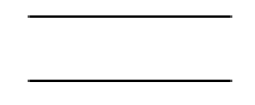
\includegraphics[width=3 in,height=1 in]{process.png}
  			\end{center}
  \end{figure}
  
  \begin{itemize}
  \item\textbf{Data Flows}
  \end{itemize}
  \par Data flows show the passage of data in the system and are represented by lines joining
  system components. An arrow indicates the direction of flow and the line is labelled by
  name of the data flow.\\
  
  \begin{figure}[h]
    	\begin{center}
    	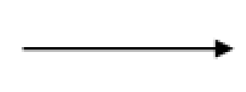
\includegraphics[width=3 in,height=1 in]{data.png}
    			\end{center}
    \end{figure}
 \newpage
 \begin{itemize}
 \item\textbf{External Entity}
 \end{itemize}
 \par External entities are outside the system but they either supply input data into the system or
 use other systems output. They are entities on which the designer has control. They may
 be an organizations customer or other bodies with which the system interacts. External
 entities that supply data into the system are sometimes called source. External entities that use the system data are sometimes called sinks. These are represented by rectangles
 in the Data flow Diagram.\\
 
 \begin{figure}[h]
   	\begin{center}
   	
   	
   		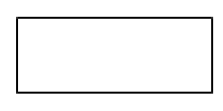
\includegraphics[width=3 in,height=1 in]{ex.png}
   			\end{center}
   \end{figure}

\textbf{LEVEL 0}

\begin{figure}[h]
  	\begin{center}
  		\includegraphics[width=3 in,height=2 in]{Dfd0.png}
  			\caption{LEVEL 0 DFD}
  			\label{LEVEL 0 DFD}
  	\end{center}
  \end{figure}
  \textbf{Description}
  \\
  \par User can ask queries and the chatbot will provide appropriate response to the user.\\
  \newpage
  \textbf{LEVEL 1}
  
  \begin{figure}[h]
    	\begin{center}
    		\includegraphics[width=5 in,height=1 in]{Dfd1.png}
    			\caption{LEVEL 1 DFD}
    			\label{LEVEL 1 DFD}
    	\end{center}
    \end{figure}
    
    \textbf{Description}
    \\
    \par User can login to the website using user name and password. After successful login user
    can input the file either in pdf format or as an e-file. Then they can ask queries related to the
    inputted document. The chatbot will reply to the query asked by the user.\\
    
    \textbf{LEVEL 2}
      
      \begin{figure}[h]
        	\begin{center}
        		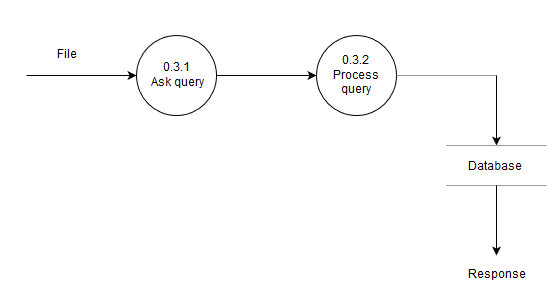
\includegraphics[width=5 in,height=2.5 in]{Dfd2.png}
        			\caption{LEVEL 2 DFD}
        			\label{LEVEL 2 DFD}
        	\end{center}
        \end{figure}
        
        \textbf{Description}
        \\
        \par When user asks query, the bot will process the query and then search the database where
        the input file is stored and appropriate answer is fetched from the database.
 \chapter{IMPLEMENTATION}
 \par Implementation is the stage in the project where the theoretical design is turned into a working system and is giving confidence on the new system for users that it will work effectively and effectively. It involves careful planning, investigation of the current system and it constraints on implementation, design of achieve the changeover, an evolution of change over method. A part from planning major task of preparing the implementation are education and training of users .The more complex system being implemented, the more involved will be the system analysis and the design effort required just for implementation.\\
 \par  The product is developed in Python environment in windows platform. This chapter may explain our implementation details.\\
 \section{ LANGUAGES AND PLATFORM USED}
\par The product is developing in Python environment and we are using MySQL for database. Microsoft SQL Server automatically tunes many of the server configuration options, therefore requiring little, if any, tuning by a system administrator. Although these configuration options can be modified by the system administrator, it is generally recommended that these options be left at their default values, allowing SQL Server to automatically tune itself based on run-time conditions.\\
\subsection{PYTHON}
Python is a widely used high-level, general purpose, dynamic programmic language. Its design philosophy emphasizes code readability, and its syntax allows programmers to express concepts in fewer lines of code than possible languages such as C++ or Java. One of the design goals of Python is that the meaning of the code is easily understood because of the very clear syntax of the language. It has a specific syntax and semantics which enables it to express computations and data manipulations which can be performed by a computer.It is designed to be highly readable. It uses English keywords frequently where as other languages use punctuation, and it has fewer syntactical constructions than other languages. Python was developed by Guido van Rossum in the late eighties and early nineties at the National Research Institute for Mathematics and Computer Science in the Netherlands. Python is derived from many other languages , including ABC, Modula-3, C, C++, Algol-68, Smalltalk, and other scripting languages.\\
\begin{itemize}
\item \textbf{Python is Interpreted:}Python is processed at runtime by the interpreter. User donot need to compile the program before executing it. This is similar to PERL and PHP.
\item \textbf{Python is Interactive:}User can actually sit at a Python prompt and interact with the interpreter directly to write the programs.
\item \textbf{Python is Object- Oriented:}Python supports Object-Oriented style or technique of programming that encapsulates code with objects.
\end{itemize}
\textbf{Features of Python includes:}
\begin{itemize}
\item \textbf{Easy-to-learn:}Python code is more clearly defined and visible to the eyes.
\item \textbf{Easy-to-read:}Python's code is more clearly defined and visible to the eyes.
\item \textbf{Easy-to-maintain:}Python's source code is fairly easy-to-maintain.
\item \textbf{Interactive Mode:}python has support for an interactive mode which allows interactive testing and debugging of snippies of code.
\item \textbf{Portable:}Python can run on a wide variety of hardware platforms and has the same interface on all platorms.
\item \textbf{Extendable:}User can add low-level modules to the Python interpreter. 
\end{itemize}
\subsection{AIML}
AIML or Artificial Intelligence Markup Language, is an XML dialect for creating natural language. AIML makes it possible to create human interfaces while keeping the implementation simple to program, easy to understand and highly maintainable.
\subsection{HTML}
HTML or Hypertext Markup Language is the standard markup language for creating web pages and web applications. HTML elements are the building blocks of HTML pages. With HTML constructs, images and other objects, such as interactive forms may be embedded into the rendered page. Web browsers receive HTML documents from a web server or from local storage and render them into multimedia web pages.
\newpage
\section{SCREENSHOTS}
\subsection{welcome page}
\begin{figure}[h]
	\begin{center}
		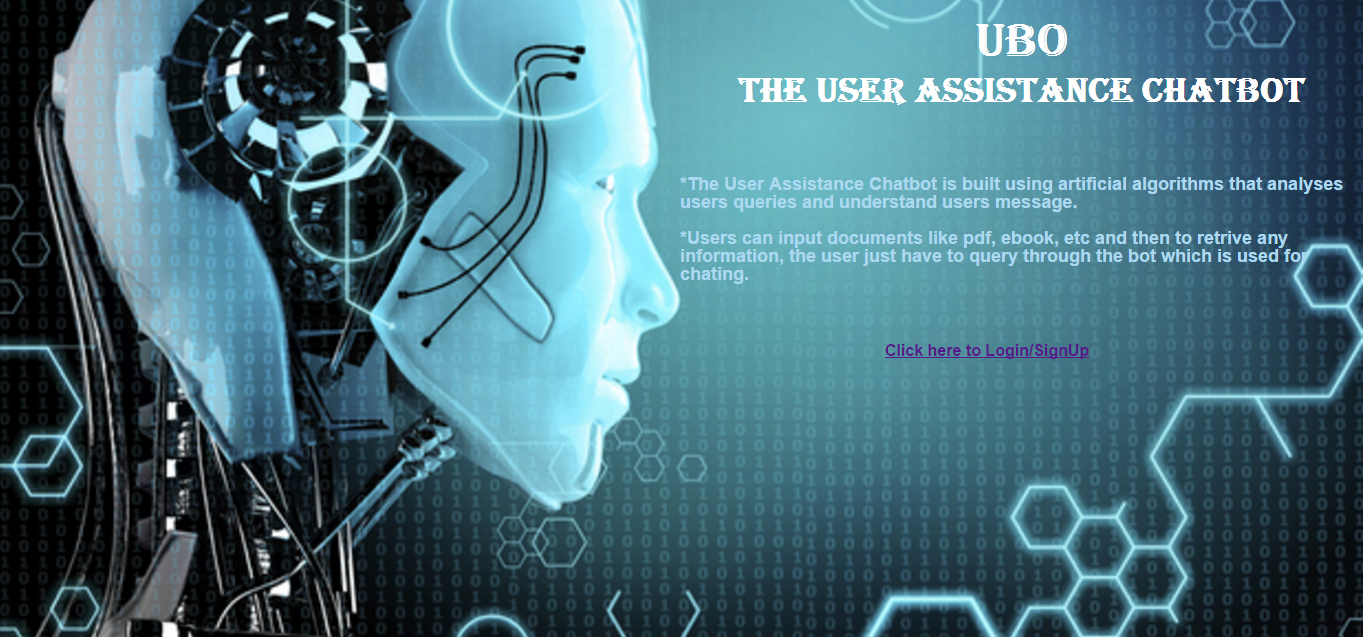
\includegraphics[width=13cm,height=7cm]{home_screen.png}
			\caption{Welcome page}
			\label{Welcome page}
	\end{center}
\end{figure}
\textbf{Description}
\par The basic informations regarding UBO is provided in this page. A new user can also get a basic knowledge about what the webpage is aimed at by reading these informations. A link to the login or sign up page is also provided in this page.



\newpage
\subsection{Sign Up}
\begin{figure}[h]
	\begin{center}
		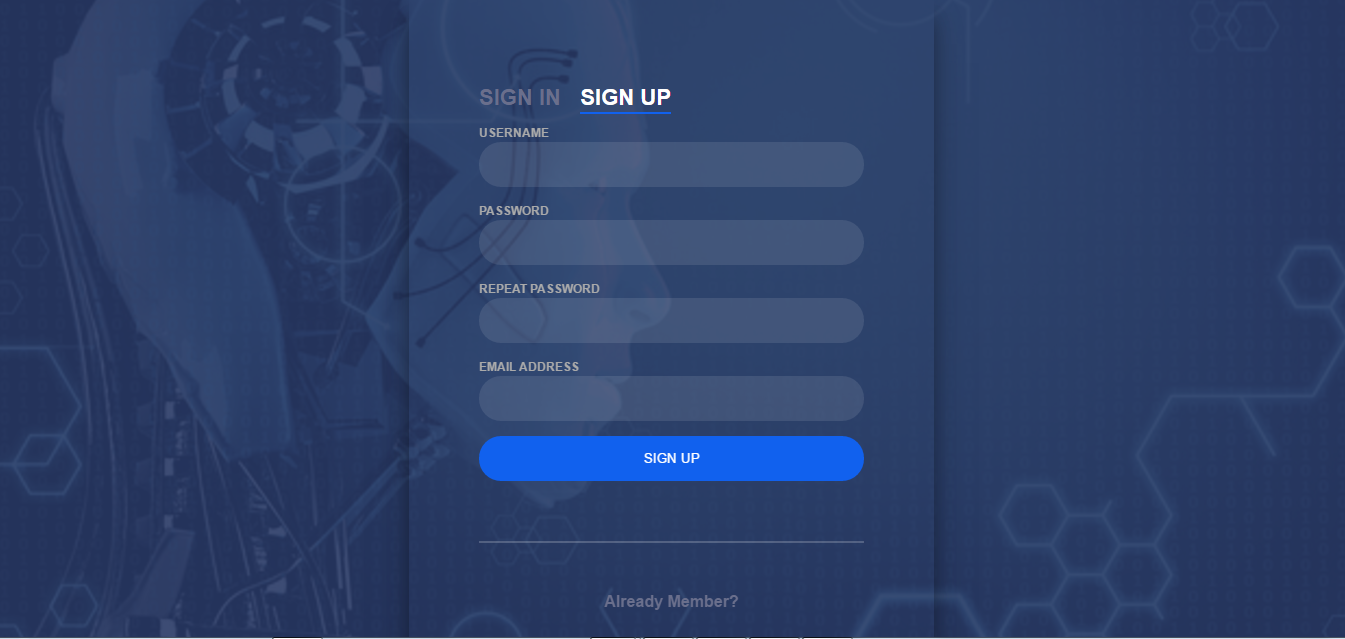
\includegraphics[width=13cm,height=7cm]{sign_up.png}
			\caption{Sign Up page}
			\label{Sign Up page}
	\end{center}
\end{figure}
\textbf{Description}
\par This page is used for a new registration. The page includes the basic informations for the registration of a new user such as name, password, email address. The link for directing the user to the sign in page is given if the user is already a member.
\newpage
\subsection{Sign In}
\begin{figure}[h]
	\begin{center}
		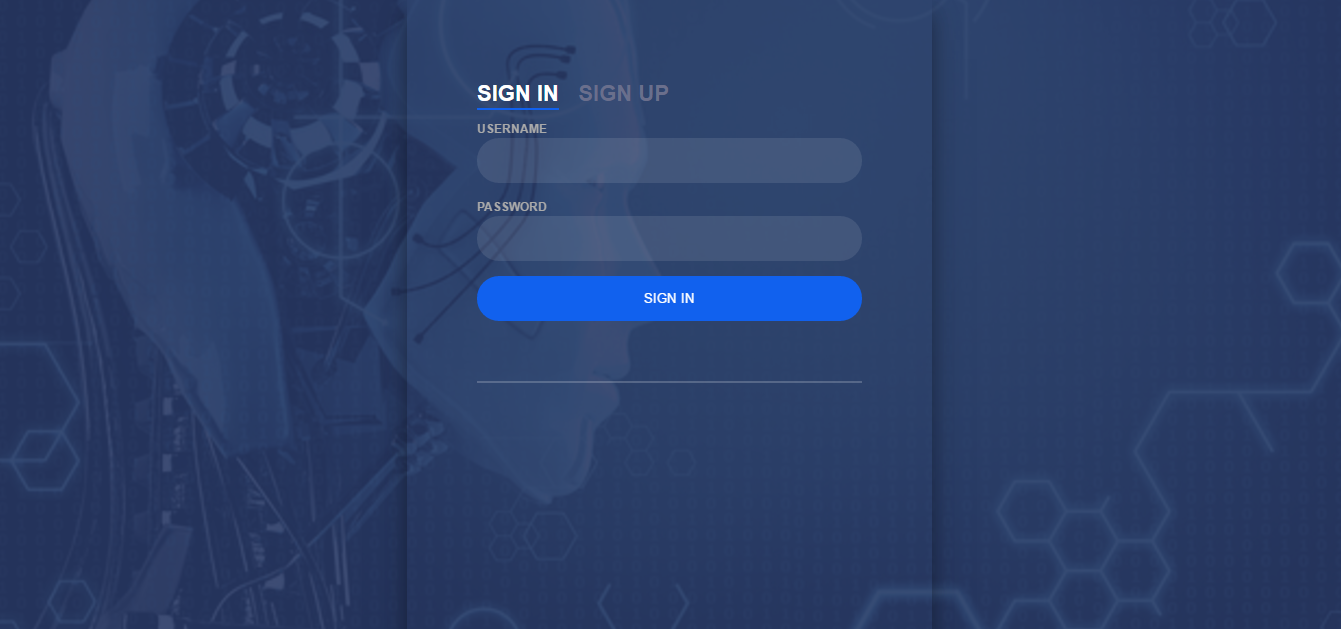
\includegraphics[width=13cm,height=7cm]{sign_in.png}
			\caption{Sign In page}
			\label{Sign In page}
	\end{center}
\end{figure}
\textbf{Description}
\par The sign in page consists of two text fields where the users need to enter their login credentials to login to UBO.

\newpage
\subsection{Home screen}
\begin{figure}[h]
	\begin{center}
		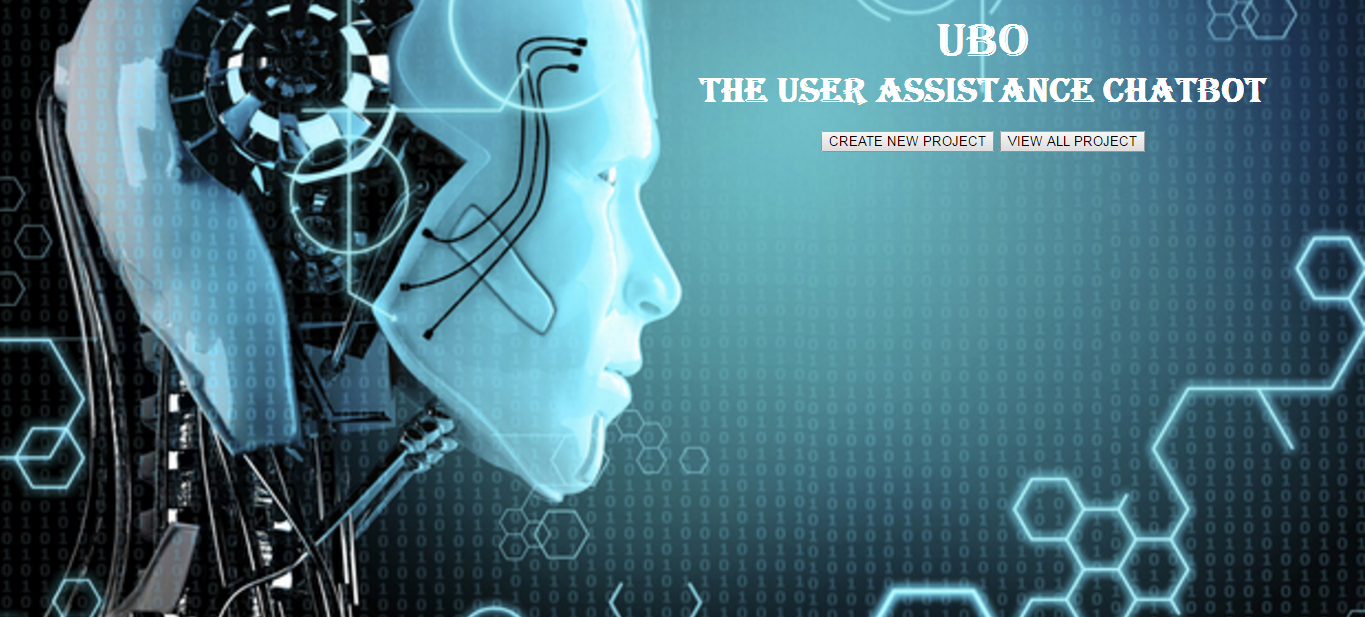
\includegraphics[width=13cm,height=7cm]{home.png}
			\caption{Home page}
			\label{Home page}
	\end{center}
\end{figure}
\textbf{Description}
\par This page has two choices. First one is to insert a new project and the second one is to view all the projects uploaded by the user.


\newpage
\subsection{File Uploading}
\begin{figure}[h]
	\begin{center}
		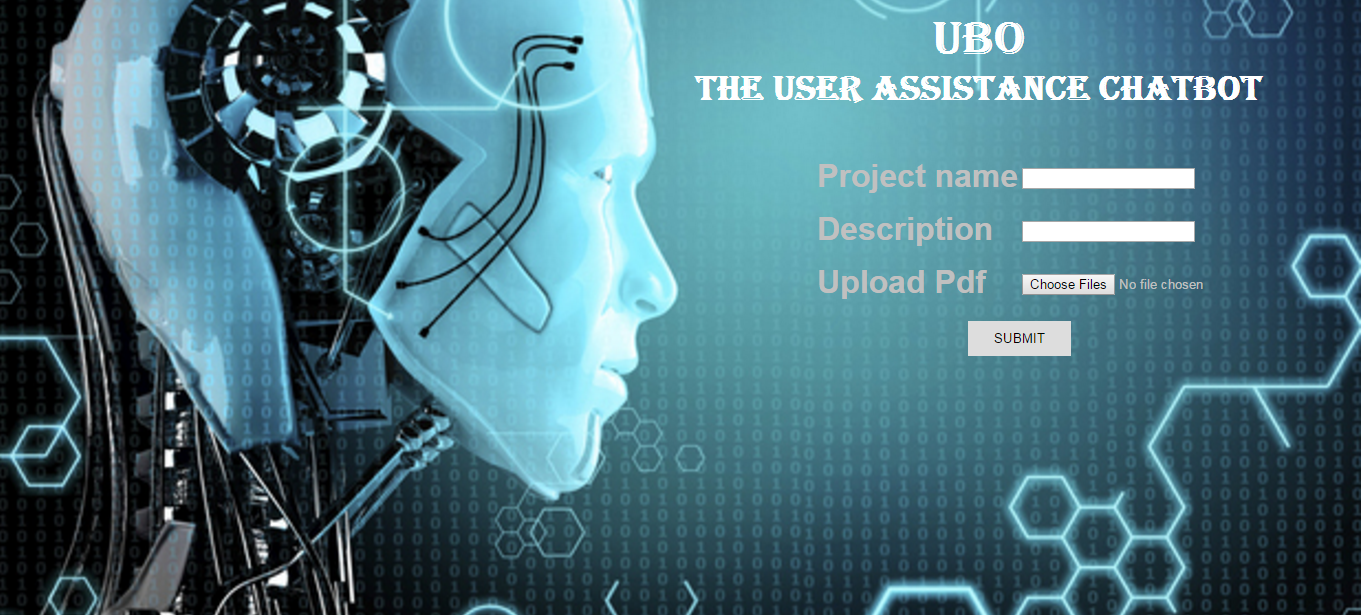
\includegraphics[width=13cm,height=7cm]{new_project.png}
			\caption{File Uploading page}
			\label{File Uploading page}
	\end{center}
\end{figure}
\textbf{Description}
\par In this page we can upload a new pdf. The page contains option to enter the project name, project description and to upload the new pdf.

\newpage
\subsection{Listing Uploaded Projects}
\begin{figure}[h]
	\begin{center}
		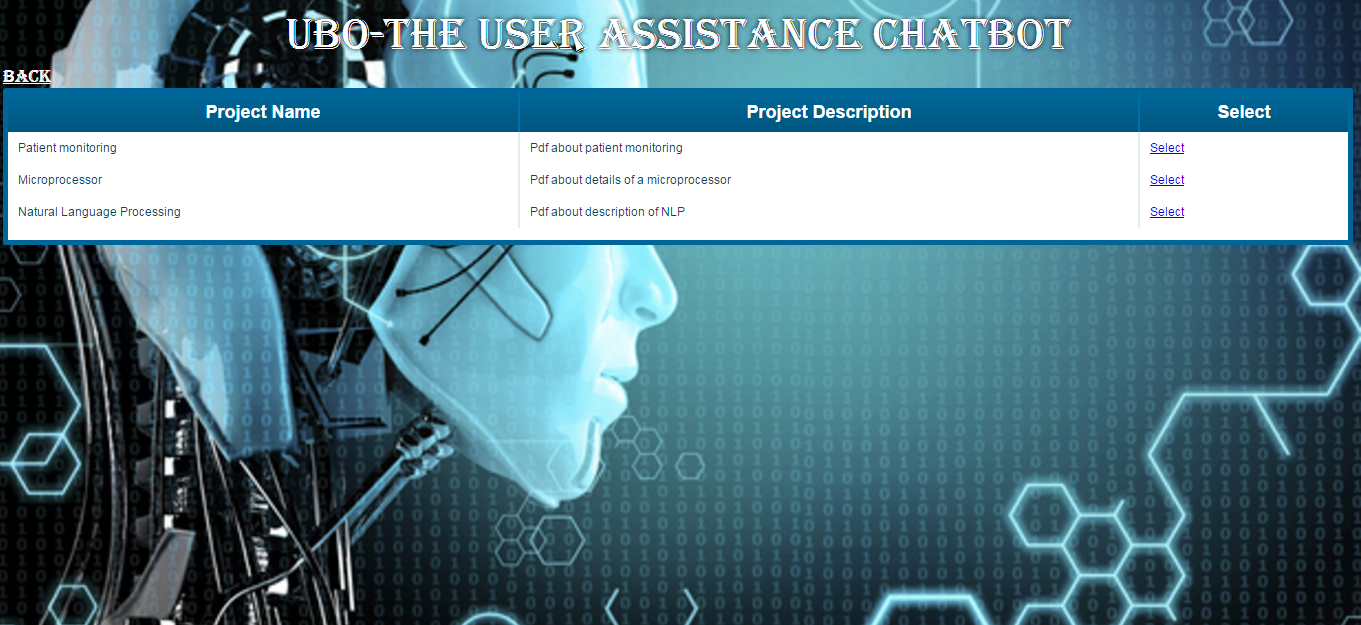
\includegraphics[width=13cm,height=7cm]{list_of_projects.png}
			\caption{Listing Projects page}
			\label{Listing Projects page}
	\end{center}
\end{figure}
\textbf{Description}
\par This page lists all the projects uploaded by he user.

\newpage
\subsection{AIML Chat}
\begin{figure}[h]
	\begin{center}
		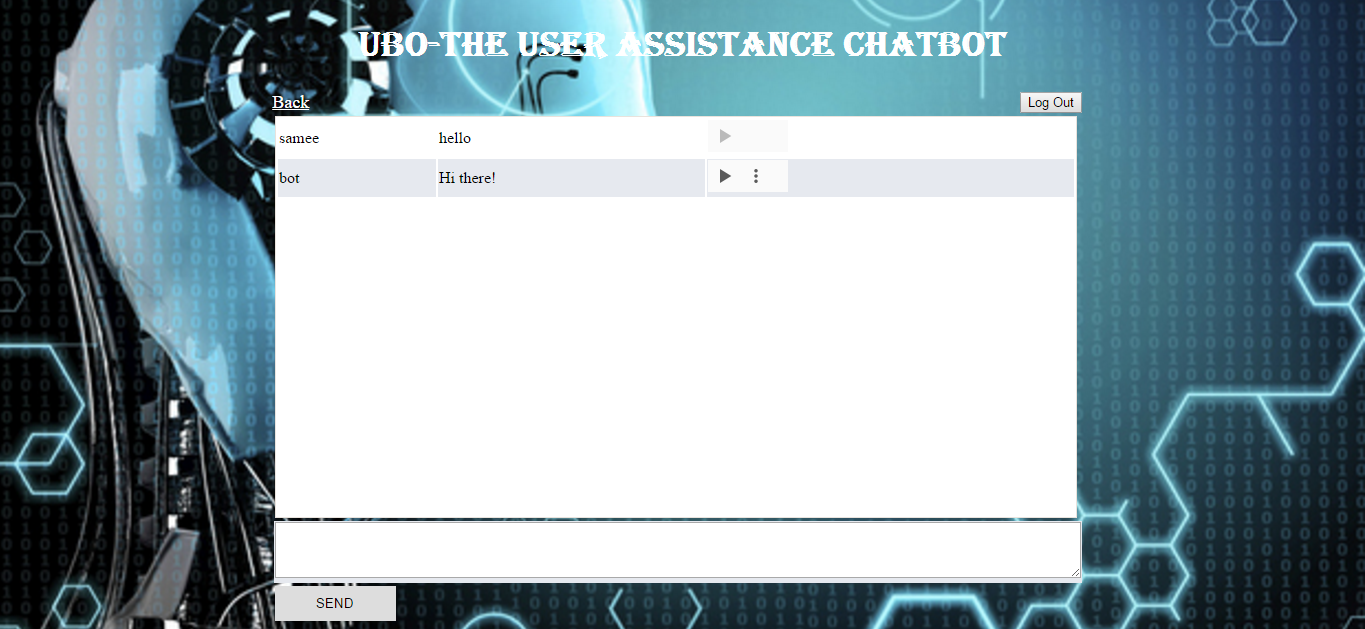
\includegraphics[width=13cm,height=7cm]{aiml_chat.png}
			\caption{AIML Chat page}
			\label{AIML Chat page}
	\end{center}
\end{figure}
\textbf{Description}
\par Here we can chat to the bot by asking casual questions like the name of bot, usual salutatons, some general questions etc.

\newpage
\subsection{Chat}
\begin{figure}[h]
	\begin{center}
		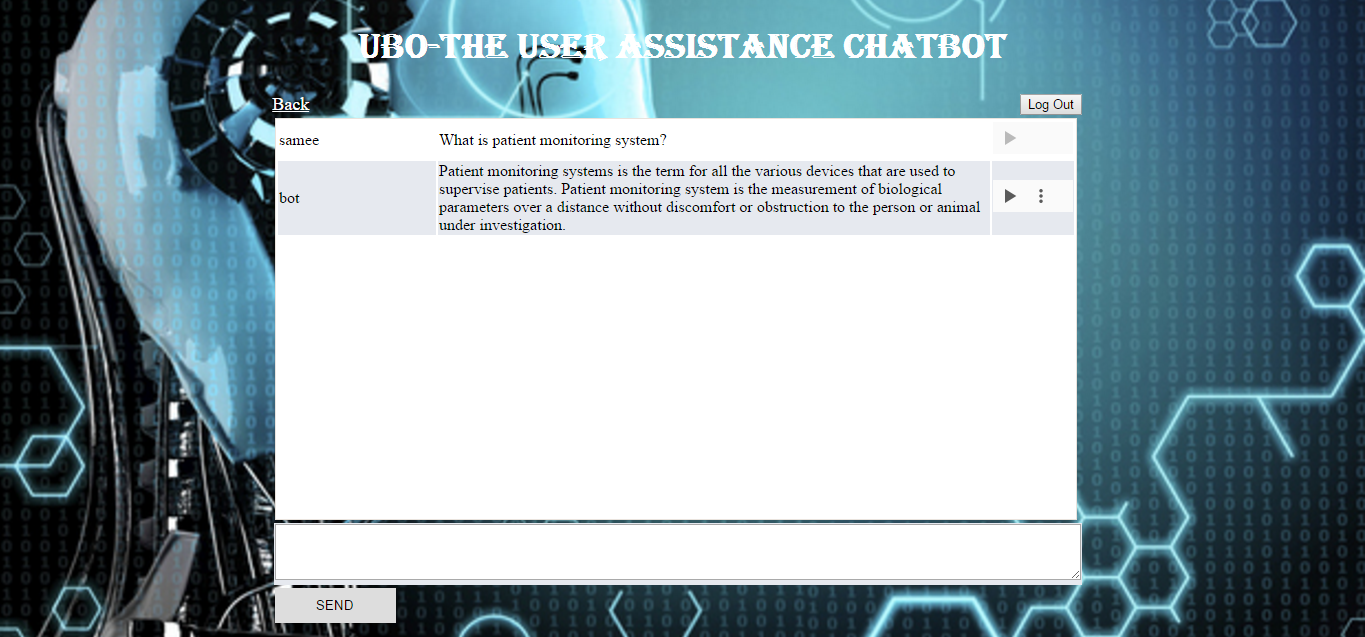
\includegraphics[width=13cm,height=7cm]{chat.png}
			\caption{Chat page}
			\label{Chat page}
	\end{center}
\end{figure}
\textbf{Description}
\par In this we can ask questions to the bot regarding the pdf which was inserted earlier.


\chapter{TESTING}
\par When a system is developed, it is hoped that it performs properly. In practice, however some errors always occur. The main purpose of testing an information system is to find the error and correct them. A successful test is one that finds an error. System testing is a critical aspect of Software Quality Assurance and represents the ultimate review of specification, design and coding. Testing is the process of executing a program with the intent of finding an as yet undiscovered error. Nothing is complete without testing. Testing is vital to the success of the system.
\par The main objectives of the system testing are:
\begin{itemize}
\item To ensure during operation the system will perform as per specification.
\item To make sure that the system meets user requirements during operation.
\item To verify that the controls incorporated in the system function as intended.
 \end{itemize}
\par If the testing conducted successfully, it will uncover errors in the software. As a secondary benefit, testing demonstrates that the software functions appear to be working according to specification and that performance requirements appear to have been satisfied.
\par The system \quotes{BerryTerminal}is tested in such a way that almost all errors that may occur are found and corrected. The test process carried out in this system includes the following:
\section{CODE TESTING}
\par In code testing the logic of the developed system is tested. For this every module of the program is executed to find any error. To perform specification test, the examination of the specifications stating what the program should do and how it should perform under various conditions. This testing was done side by side with coding. This examines the logic of the program. In java special test cases are used for testing the code. Every part of the program was tested in this phase.
\section{PASSWORD TESTING}
\par This is done for user authentication. This process ensures security of the system thus avoiding unauthorized access to the system. When the user enters the username and password, checking it with the already registered usernames and passwords will validate him. If it matches then only the user is allowed to enter in to the system. Otherwise he is denied access and thereby strong security is provided. The password checking was done for the system. Only registered users were able to login.
\section{UNIT TESTING}
Unit testing is undertaken after a module has been coded and reviewed. Before carrying this testing, the unit test cases have to be designed and the test environment for the unit under test has to be developed. The various test cases are driver and stub modules. The main objective is to determine the correct working of the individual modules. During the testing each module is isolated from other modules and individually unit tested. It involves a precise definition of the test cases, testing criteria, and management of test cases. The modules that are tested include Client Terminal, Network Management and Server Management module.
 \section{INTEGRATION TESTING}
System testing does not test the software as a whole, but rather than integration of each module in the system. The primary concern is the compatibility of individual modules. One has to find areas where modules have been designed with different specifications of data lengths, type and data element name. Testing and validation are the most important steps after the implementation of the developed system. The system testing is performed to ensure that there are no errors in the implemented system. The software must be executed several times in order to find out the errors in the different modules of the system. Each of the modules were integrated together and subjected to testing.
\section{VALIDATION TESTING}
Validation refers to the process of using the new software for the developed system in a live environment i.e., new software inside the organization, in order to find out the errors. The validation phase reveals the failures and the bugs in the developed system. It will come to know of the practical difficulties the system faces when operated in the true environment. Validation test was performed in the Login section. By testing the code of the implemented software, the logic of the program can be examined. A specification test is performed to check whether the specifications stating the program are performing under various conditions. Apart from these tests, there are some special tests conducted which are given below:
\begin{itemize}
\item \textbf{Peak load test} This determines whether the new system will handle the volume of activities when the system is at the peak of its processing demand. The test has revealed that the new system is capable of handling the demands at the peak time.
\item \textbf{ Storage testing }  This determines the capacity of the new system to store transaction data on a disk or on other files. The proposed software has the required storage space available. 
\item \textbf{ Performance time testing } This test determines the length of the time used by the system to process transaction data.
 

\end{itemize}
 \section{SYSTEM TESTING}
 \par After all units of a program have been integrated together and tested system testing is taken up. It is same for both procedural and object oriented programming. System tests are designed to validate a fully developed system to assure that it meets its requirements. The system test cases can be classified into performance and functionality test cases. The functionality test cases are designed to check whether the software satisfies the functional requirements as documented in the SRS document. The performance tests on the other hand test the conformance of the system with non-functional requirements of the system.
 \section{OUTPUT TESTING}
 \par After the performance of unit testing, the next step is output testing. No system would be useful if it does not produce the required output in the specific format, thus output format on the screen is found to be correct when the format was designed in the system phase according to the user need.
 \par The maintenance of software is the time period in which software product performs useful works. Maintenance activities involve making enhancement to software product, adapting product to new environment and correcting problems. It includes both the improvement of the system function.  
\par It may involve the continuing involvement of a large proportion of computer department resources. The main task may be to adapt existing system in a changing environment. System should not be changed casually following informal requests. To avoid unauthorized amendments, all requests for change should be channelled to a person nominated by management. The nominated person has sufficient knowledge of the organization’s computer based systems to be able to judge the relevance of each proposed change. 
\par No annual costs for support or maintenance are required. Ofcourse, the individual system components come with limited warranty from the manufacturers, i.e., the PC, camera, etc. There is no obligation to purchase or pay for any extended maintenance or support.
\section{GOAL OF TESTING}
\par Many users may use our project. So the project designer must test all the modules of the project. The main goal of our project is, whenever user uses our project, it should run without any error.
\section{PASS/FAIL CRITERIA}
\par The pass/fail criteria specifies a set of constraints whose satisfaction leads to approval or disapproval of the proper functioning of the system .
\section{PASS CRITERIA}
\par The system must meet all the functional and non-functional requirements. Pass all the test cases, get the expected response, and get acceptable performance to be tested pass.
\begin{itemize}
\item User can login and submit pdf
\item  User can ask queries and the system responds.
\item Periodic update of database
\end{itemize}
\section{FAIL CRITERIA}
\par If one of the following situations happens, the system is considered to fail:
\begin{itemize}
\item  User cannot login
\item  Database updation failure
\item  Human error
\end{itemize}


\newpage
\section{TEST REPORT}
\par The detailed test reports prepared for each function. A sample test report is given below:
\\
\begin{table}[]
\centering
\caption{Test Report}
\label{Test Report}
\begin{tabular}{|l|l|}
\hline
Name                                                                                & User Assistance Chatbot                                              \\ \hline
Version                                                                             & 1.0                                                                  \\ \hline
Author                                                                              & Anjali Krishna, K M Sameera, Lekshmi Lal D, Sumayya V A              \\ \hline
Approved By                                                                         & Self                                                                 \\ \hline
Date                                                                                & Thursday, 10th March 2017                                            \\ \hline
Role                                                                                & User can operate the system                                          \\ \hline
Prerequisite                                                                        & The user is logged into the system                                   \\ \hline
User/Actor                                                                          & System Response                                                      \\ \hline
Login                                                                               & User can enter their username and password to login.                 \\ \hline
Run Applications                                                                    & After successful authentication, the user can run those application. \\ \hline
Handle User Data                                                                    &                                                                      \\ \hline
                                                                                    &                                                                      \\ \hline
\begin{tabular}[c]{@{}l@{}}The test project\\ was successfully\\ saved\end{tabular} &                                                                      \\ \hline
\end{tabular}
\end{table}
\par Test case preparation helps the user and the developer to find and fix the errors easily and in advance. Berry Terminal is well tested with the proper test cases and thus passed a better unit test. Elaborated test cases also prepared subjected the system for thorough testing. The test cases prepared are in the following format.\\


\section{BLACKBOX TESTING}
\par Black-box testing is a method of software testing that examines the functionality of an application without peering into its internal structures or workings. Test case preparation helps the user and the developer to find and fix the errors easily and in advance. Disease-Symptom Analyser using MapReduce is well tested with the proper test cases and thus passed a better unit test.\\
 The test cases prepared are in the following format:\\
 \\

\begin{table}[]
\centering
\caption{Test Cases}
\label{Test Cases}
\begin{tabular}{|l|l|l|l|l|l|}
\hline
Test & Usecase step & \begin{tabular}[c]{@{}l@{}}Action performed\\ /User input\end{tabular} & \begin{tabular}[c]{@{}l@{}}Expected Result\\ /system response\end{tabular} & \begin{tabular}[c]{@{}l@{}}Actual          \\    result\end{tabular} & \begin{tabular}[c]{@{}l@{}}Do expected and \\ actual result cor-\\ respond\end{tabular} \\ \hline
1    & User         & \begin{tabular}[c]{@{}l@{}}Enter username \\ and password\end{tabular} & \begin{tabular}[c]{@{}l@{}}View sucess\\ page\end{tabular}                 & As Expected                                                          & Yes                                                                                     \\ \hline
2    & User         & Ask queris                                                             & \begin{tabular}[c]{@{}l@{}}View the \\ answer\end{tabular}                 & As Expected                                                          & Yes                                                                                     \\ \hline
3    & Bot          & \begin{tabular}[c]{@{}l@{}}Replies to the \\ user\end{tabular}         & \begin{tabular}[c]{@{}l@{}}View the \\ answer\end{tabular}                 & As Expected                                                          & Yes                                                                                     \\ \hline
4    & User         & Logout                                                                 & \begin{tabular}[c]{@{}l@{}}View the login\\ page\end{tabular}              & As Expected                                                          & Yes                                                                                     \\ \hline
\end{tabular}
\end{table}


\chapter{FUTURE SCOPE}
\par In the proposed system all details about the system is designed into an application. It is designed as a web based application, which will work smoothly on any computer system with internet connection. For using/operating the application, there will be no need of additional staff. Any person with basic computer knowledge can use this application. The applications own operational staff is found to be sufficient and efficient to handle the system. Once the system is hosted on the web, the system will be automatically operated. Nowadays people are familiar with internet and e-mail, and hence, they can easily use the options from the home page of the new system. So the proposed system is operationally feasible. The document automations of software is also supported by a powerful database where the documents are arranged, making updates and collaboration easy and fast. The basic steps in application processing is same everywhere, and hence the extended version of this system be used in advanced areas too.  The existing chatbots are ELIZA, ALICE, etc. They are just used for chatting purposes. Currently the user has to read a large document for getting any information from it. There is a wastage of time and effort. The chatbot is trained in such a way that it answers to the queries of user related to the inputed document. The user don’t have to waste the time by reading whole document instead the bot will answer the queries. It reduces the burden of user who has to read a large document. I The output will be available in the form of both text and speech. The system will provide precise answers to the queries.




\chapter{CONCLUSION}
Chatbots are computer programs that interact with users using natural languages. Just as people use language for human communication, chatbots use natural language to communicate with human users. A chatbot is one of the easiest way to fetch information from a system without having to think for proper keywords to look up in a search engine or browse several web pages to collect information, users can easily type their query in 
natural language and retrieve information. This chatbot has built-in knowledge-base, conversational abilities, real-time support, and human visual look. It can act as a great virtual assistant.
\par The user assistance chatbot is built using Artificial Intelligence. The system is aimed to work on web based platform. It answers to the queries of a user related to the inputted document. The system helps in saving time and effort of the user. When the user will ask a query, this query will be matched against the various patterns present in the database and the template corresponding to that pattern will be returned in form of text and speech to the user.\\  
 

\chapter{GLOSSARY}
\begin{itemize}
\item\textbf{ AIML}: Artificial Intelligence Markup Language
\item\textbf{ COCOMO}: Constructive Cost Estimation Model
\item\textbf{ DFD}: Data Flow Diagram
\item\textbf{ KLOC}: Kilo Lines Of Code
\item\textbf{ LOC}: Lines Of Code
\item\textbf{ HTML}: Hypertext Markup Language
\item\textbf{ HTTP}: Hyper Text Transfer Protocol
\item\textbf{ GUI}: Graphical User Interface
\item\textbf{ OS}: Operating System
\item\textbf{ RAM}: Random Access Memory
\item\textbf{ UML}: Unified Modeling Language
\end{itemize}
\renewcommand{\bibname}{REFERENCES}
\begin{thebibliography}{999}
\addcontentsline{toc}{chapter}{\hspace{0.2in} REFERENCES}
 \bibitem {r1} S.J.du Preez,M.Lall,S.Sinha,"An Intelligent Web Based Voice Chat Bot"\textit{International Conference on Information Technology}.
 \bibitem {r2} Salto Martinez Rodrigo,Jacques Garcia Fausto Abraham, "Development and Implementation of a Chat Bot in a Social Network "\textit{2012 Ninth International Conference on Information Technology }.
 \bibitem{r3} Prof.Nikita Hatwar,Ashwini Patil, Diksha Gondane, "AI Based chatbot"\textit{International journal of emerging trends in engineerind and basic science}.
 \bibitem{r4} Donghui Feng, Erin Shaw, Jihie Kim, Eduard Hovy,"An intelligent discussion bot for answering student queries in threaded discussions"\textit{AIED 2005}
 \bibitem{r5}ALICE. \textit{http://www.alicebot.org/}
\end{thebibliography}

	



\end{document}
